% !TEX root = paper.tex
\iflong
\else
\vspace{-2mm}
\fi
\section{Preferred Replacement path avoids $t_s$}

\label{sec:avoids}


Handling preferred replacement paths that avoid $t_s$ turns out to be a challenging and unexplored case. For better exposition, we will first solve the problem for the case when $\sigma=1$, that is there is only one source.
Let $\RR$ be the set of all preferred replacement paths from $s$ to $t$ that do not pass through $t_s$. We make  two important observations:

\begin{enumerate}[noitemsep,nolistsep]

\item The size of $\RR$ is $ O(\sqrt n)$.

\item Preferred replacement paths in $\RR$ avoid one contiguous sub path of $st$.

\end{enumerate}

\noindent Few remarks are in order. If the preferred replacement paths in $\RR$ were disjoint, then bounding the size of $\RR$ is easy. However, we are able to bound the size of $\RR$ even if paths are intersecting.  The second observation implies that we can build a balanced binary search tree containing paths in $\RR$. Each node in this tree will contain a preferred replacement path $P$. The key for each node will be the start and end vertex of the sub path $P$ avoids.  We will use this BST to find an appropriate replacement path that avoids an edge $e$.

\begin{definition}(Detour of a replacement path)
Let $P$ be a preferred replacement path avoiding an edge $e$ on $st$ path. Then detour of $P$ is defined as, $\DET(P) := P \setminus st$. That is, detour is a path the leaves $st$ before $e$ till the point it merges back to $st$ again.
\end{definition}

\begin{comment}
\begin{lemma}
\label{lem:prop}
Let $P$ be a replacement path in $\RR$ that avoids $u$ on $st_s$ path. Then
 $P$ can merge back to $st$ path just once.
\end{lemma}
\begin{proof}
Since $P$ is a replacement path from $s$ to $t$ avoiding $u$, it necessary has to merge somewhere on path $st$. Assume that $P$ merges back at $w$ on $st$ path. Note that $w$ cannot lie before $u$ on $st$ path as the sub-path $sw$ of the $st$ path is the shortest path from $s$ to $w$. This implies that $w$ lies after $u$ on $st$ path. After merging at $w$, $P$ can continue on the sub path $wt$ (of path $st$) to reach $t$, as this is the shortest path from $w$ to $t$.
\end{proof}
\end{comment}
\noindent Since our  replacement path $P$  also avoids $t_s$, the following lemma is immediate by the definition of preferred path.

\begin{lemma}
Let $P$ be a preferred replacement path in $\RR$ that avoids $e$ and $t_s$ on
$st$ path, then (1) $\DET(P)$ cannot merge back to $st_s$ path and (2) $\DET(P)$ is a contiguous path.
\end{lemma}
\begin{lemma}
\label{lem:avoids}
Let $P,P' \in \RR$ avoid $e$ and $e'$ respectively on $st_s$ path. Also assume that $e$ is closer to $s$ than $e'$. Then
(1)  P avoids $e'$  (2) $\DET(P')$ starts  after $e$ on $st_s$ path and (3) $|P| > |P'|$.

\end{lemma}

\iflong
  \begin{proof}

  \noindent (1) $P$ diverges from $st_s$ path above $e$. Since $P
  \in \RR$, it   merges back on $t_st$ path only. Since $e,e'
  \in st_s$ (we are in {\em far} case) and $e$ is closer to $s$ than $e'$, this implies
  that $P$ also avoids $e'$.

  \noindent (2) Assume that  $\DET(P')$ starts above $e$ on
  $st_s$ path. This implies that both $P$ and $P'$ avoid $e$
  and $e'$. But then, our algorithm will choose one of these two paths as a preferred path that avoids both $e$ and $e'$.  Thus,
  we arrive at a contradiction as there are two different preferred replacement paths avoiding $e$ and $e'$.

  \noindent (3) Since $P$  avoids $e'$ (by (1)) and $\DET(P')$ starts after $e$ (by (2)), $P'$ is the preferred path to avoid $e'$ only if $|P'| < |P|$ (else $P$ would be the preferred path as it leaves the $st$ path earlier than $P'$).



  \end{proof}
\fi

\noindent The converse of the third part of the lemma is also true. Since we will be using it in future, we prove it now.

\begin{lemma}
\label{lem:avoidreverse}

Let   $P$ and $P'$ be two preferred replacement paths that avoid $e$ and $e'$ on $st$ path respectively. If $|P| > |P'|$, then $e$ is closer to $s$ than $e'$.
\end{lemma}

\iflong
  \begin{proof}
  Assume for contradiction that $e'$ is closer to $s$ than $e$. Since the replacement path $P'$ has to diverge from $st$ before $e'$ and merge again only in $t_st$,  $P'$ also avoid $e$. But then $P'$ should be the replacement path for avoiding $e$ too, as $|P'| < |P|$, a  contradiction.
  \end{proof}
\fi
\iflong
\else
\begin{figure}[hpt!]
\centering
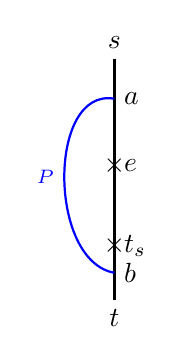
\begin{tikzpicture}[scale=1.7]

\definecolor{dgreen}{rgb}{0.0, 0.5, 0.0}
\begin{scope}[xshift=0cm]
\coordinate (s) at (0,1.8);
\coordinate (t) at (0,0);
\coordinate (ts) at (0,0.4);
\coordinate (b) at (0,.2);

\coordinate (a) at (0,1.5);
\coordinate (v) at (0,1);

\draw[thick](s)--(t);
\node[above] at (s){$s$};
\node[below] at (t){$t$};
\node[right] at (a){$a$};
\node[right] at (b){$b$};



\draw[blue,thick] (a) to[out=170,in=170] node[pos=0.5,left]
{\scriptsize  $P$}  (b);
\node at (v){$\times$};
\node[right] at (v){$e$};

\node at (ts){$\times$};
\node[right] at (ts){$t_s$};
\end{scope}

\end{tikzpicture}

\caption{$\DET(P)$ does not intersect detour of any path in $(>P)$}
\label{fig:singlefirstcase}
\end{figure}

\fi
\noindent By Lemma \ref{lem:avoids}{\small(3)}, we know that all preferred replacement
paths in $\RR$ have different lengths. In fact, it is the main reason we defined a preferred replacement path. We can thus arrange
these paths   in decreasing order of their lengths. Thus, we get the following corollary.
\begin{corollary}
\label{cor:arrange}
 Given a set $\RR$ of preferred replacement paths from $s$ to $t$ (that also avoid $t_s$), we can arrange  paths in decreasing order of their lengths.
\end{corollary}

\noindent Given a path $P \in \RR$, let $(<P)$ be the set of all preferred replacement paths with length less than $P$. Similarly, let $(>P)$ be the set of all preferred replacement paths with length greater than $P$.   If $P$ avoids $e$, then by Lemma \ref{lem:avoidreverse}, it also avoids all  edges avoided by paths in $(<P)$.  By Lemma \ref{lem:avoids}, for any path $P' \in (<P)$, $\DET(P')$ starts after $e$ on $st_s$ path.
We will now show a simple but important property of a path $P$ in $\RR$.

\begin{lemma}
\label{lem:length}
Let $P \in \RR$ be the shortest path from $s$ to $t$ avoiding $e$ such that $|P| = |st| +\ \ell$ where $\ell \ge 0$, then the size of the set $(<P)$ is $\le \ell$.
\end{lemma}
\iflong
  \begin{proof}
  Since a path in $(<P)$ avoids some edge in $st$ path, its length has to be $\ge |st|$. By Corollary \ref{cor:arrange},
  all paths in $\RR$, and thus $(<P)$ have different lengths. But the length of paths in $(<P)$ is less than the length of $P$.
  Thus, there can be atmost $\ell$ paths in $(<P)$.
  \end{proof}
\fi

\begin{definition}
\label{def:unique}
(Unique path of $P$) Let $\UNQ(P)$ be the prefix of\ $\DET(P)$ which does not intersect with any detours in $\cup_{P' \in (>P)} \DET(P')$.
\end{definition}
%Note that $\UNQ(P)$ can be an empty path too.
We now arrange all  preferred replacement paths in $\RR$ in decreasing order of their lengths. Assume that we are processing a path $P$ according to this ordering such that $P$ avoids $e$ on $st$ path. If $|\UNQ(P)| \ge \sqrt n$, then we have associated $O(\sqrt n)$ vertices on $\UNQ(P)$ to $P$. Else $\UNQ(P) < \sqrt{n}$ and we have the following two cases:

\iflong
\else
\vspace{-2mm}
\fi
\subsection{   $\DET(P)$ does not intersect with  detour of any path in $(>P)$}
\label{subsec:singlecaseone}
\iflong
\begin{figure}[hpt!]
\centering
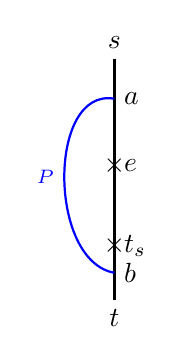
\begin{tikzpicture}[scale=1.7]

\definecolor{dgreen}{rgb}{0.0, 0.5, 0.0}
\begin{scope}[xshift=0cm]
\coordinate (s) at (0,1.8);
\coordinate (t) at (0,0);
\coordinate (ts) at (0,0.4);
\coordinate (b) at (0,.2);

\coordinate (a) at (0,1.5);
\coordinate (v) at (0,1);

\draw[thick](s)--(t);
\node[above] at (s){$s$};
\node[below] at (t){$t$};
\node[right] at (a){$a$};
\node[right] at (b){$b$};



\draw[blue,thick] (a) to[out=170,in=170] node[pos=0.5,left]
{\scriptsize  $P$}  (b);
\node at (v){$\times$};
\node[right] at (v){$e$};

\node at (ts){$\times$};
\node[right] at (ts){$t_s$};
\end{scope}

\end{tikzpicture}

\caption{$\DET(P)$ does not intersect detour of any path in $(>P)$}
\label{fig:singlefirstcase}
\end{figure}

\fi
    Let $\DET(P)$ start at $a$ and end at $b$ -- the vertex where it touches
    $t_st$ path. Let $ab$ denote the
path from $a$ to $b$ on $P$. By our assumption $\UNQ(P) = ab$ and $|ab| < \sqrt n$.
    By Lemma \ref{lem:avoids}, all  replacement paths in $(<P)$ pass through $e$
    (as detour of these replacement paths start below $e$) and by Lemma \ref{lem:avoidreverse},
    these replacement paths avoid edges that are closer to $t$ than $e$. We can view the
    replacement paths as if they are starting from the vertex $a$. That is, consider  paths
    $\{P\setminus sa\} \cup \{ P'\setminus sa | \ P' \in (<P)\}$. These replacement
    paths avoid edges in $at$.   $|P \setminus sa| = |ab| +  |bt| \le |ab|\ + |at| < |at| + \sqrt n$.
    Applying Lemma \ref{lem:length}, we infer that the number of paths in $\{ P'\setminus
sa | P' \in (<P)\}$ is $\le \sqrt n$

\iflong
\else
\vspace{-2mm}
\fi
\subsection{$\DET(P)$ intersects with  detour of a path in $(>P)$}
\label{subsec:singlecasetwo}
Assume that $P$ first intersects with $P' \in (>P)$. Let $P'$ avoid $e'$ and $\DET(P')$ start at $a'$ and end at $b'$ (see Figure \ref{fig:singlesecondcase}). Let us assume that $\DET(P)$ starts at $a$ and it intersects $\DET(P')$ at $c$. This implies that $\UNQ(P) = ac$.

\noindent Consider the path $sa' \conc a'c \conc ca \conc at$. We claim that this path avoids $e'$. This is due to the fact that by Lemma \ref{lem:avoids}, $\DET(P)$
starts after $e'$ on $st$ path. So, $ca$ and $at$ avoids $e'$. Since $P' = sa' \conc a'c \conc cb' \conc b't$, length of $P'$ must be $\le$ length of the alternate path. Thus,\\
\begin{tabular}{llll}
 & $|sa'| +  |a'c|
+ |cb'| + |b't|$  & $\le$ &$|sa'| + |a'c| + |ca|  + |at|$\\
$\implies$& $
|cb'| + |b't|$ & $\le$ & $|ca|  + |at|$   \\
$\implies$& $|ac| +
|cb'| + |b't|$ & $\le$ &   $2|ca|  + |at|$

\end{tabular}

\begin{figure}[hpt!]
\centering
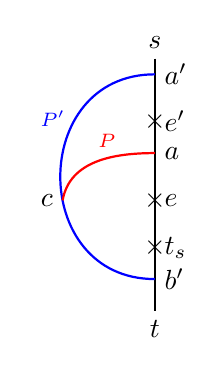
\begin{tikzpicture}[scale=2]

\definecolor{dgreen}{rgb}{0.0, 0.5, 0.0}
\begin{scope}[xshift=0cm]
\coordinate (s) at (0,1.6);
\coordinate (t) at (0,0);
\coordinate (ts) at (0,0.4);
\coordinate (b1) at (0,.2);

\coordinate (a1) at (0,1.5);
\coordinate (a) at (0,1);
\coordinate (v) at (0,0.7);
\coordinate (v1) at (0,1.2);
\coordinate (c) at (-0.585,0.7);

\draw[thick](s)--(t);
\node[above] at (s){$s$};
\node[below] at (t){$t$};
\node[right] at (a1){$a'$};
\node[right] at (a){$a$};
\node[right] at (b1){$b'$};
\node[left] at (c){$c$};


\draw[blue,thick] (a1) to[out=180,in=180,distance=.8cm] node[pos=0.3,left]
{\scriptsize  $P'$}  (b1);

\draw[red,thick] (a) to[out=180,in=80]
node[pos=0.4,above]
{\scriptsize  $P$}  (c);

\node at (v1){$\times$};
\node[right] at (v1){$e'$};

\node at (v){$\times$};
\node[right] at (v){$e$};

\node at (ts){$\times$};
\node[right] at (ts){$t_s$};
\end{scope}

\end{tikzpicture}

\caption{$\DET(P)$ intersects first with $\DET(P')$ at $c$ where  $P'
\in (>P)$.}
\label{fig:singlesecondcase}
\end{figure}

On the left hand of the inequality, we  have a path from $a$ to $t$ avoiding $e$. So, its length should be $\ge$ length of the preferred path $P \setminus sa$. Thus $|P \setminus sa| \le  2|ca|  + |at| \le 2\sqrt n\
+\ |at|$. By Lemma \ref{lem:avoids},
all  replacement paths in $(<P)$ pass through $e$ (as
detour of these replacement paths start below $e$) and by
Lemma \ref{lem:avoidreverse}, these replacement paths avoid
edges that are closer to $t$ than $e$. We can view the
replacement paths as if they are starting from the vertex $a$.
That is, consider  paths $\{P\setminus sa\} \cup \{ P'\setminus
sa | P' \in (<P)\}$. Applying lemma \ref{lem:length}, we infer that the number of
paths in $\{ P'\setminus
sa | P' \in (<P)\}$ is $\le 2 \sqrt n$.


Our arguments above point to the following important observation: {\em Once we find a replacement path in $\RR$ with unique path length $< \sqrt n$, then there are at most 2$\sqrt n$ replacement paths in $\RR$ left to process.}
Since there can be at most $\sqrt n$ paths in $\RR$ with unique path length $\ge \sqrt n$, we have proven the following lemma:

\begin{lemma}
\label{lem:sizeR}
%Let $\RR$ be all the replacement paths from $s$ to $t$ whose detour avoids $t_s$, then
$|\RR| = O(\sqrt n)$.
\end{lemma}

We now build a data-structure which will exploit Lemma \ref{lem:sizeR}.
However, we need another key but simple observation. By Lemma \ref{lem:avoids}, if $|P| > |P'|$, then $\DET(P')$ starts below the edge avoided by $P$. This lemma implies that $\DET(P')$ starts below all  edges avoided by $P$. Thus $P$ avoids some contiguous path in $st_s$ and detour of all replacement paths in $(<P)$ start below the last edge (which is closer to $t_s$) in this subpath. Thus, we have proved the second key lemma:

\begin{lemma}
\label{lem:contiguous}

A replacement path $P$ avoids a contiguous subpath of $st$.
\end{lemma}
\iflong
\else

\begin{figure}[hpt!]

\centering
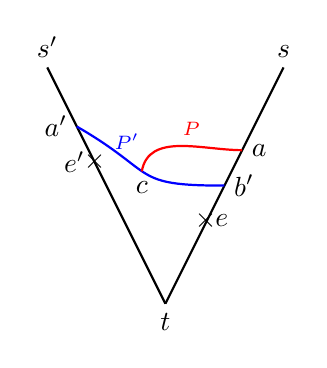
\begin{tikzpicture}[scale=1.5]

\definecolor{dgreen}{rgb}{0.0, 0.5, 0.0}
\begin{scope}[xshift=0cm]
\coordinate (s) at (-1,2);
\coordinate (s1) at (1,2);
\coordinate (t) at (0,0);
\coordinate (ts) at (0,0.4);
\coordinate (b1) at (0.5,1);

\coordinate (a1) at (-0.75,1.5);
\coordinate (a) at (0.65,1.3);
\coordinate (v) at (0.34,0.7);
\coordinate (v1) at (-0.6,1.2);
\coordinate (c) at (-0.2,1.12);

\draw[thick](s)--(t);
\draw[thick](s1)--(t);
\node[above] at (s){$s'$};
\node[above] at (s1){$s$};
\node[below] at (t){$t$};
\node[left] at (a1){$a'$};
\node[right] at (a){$a$};
\node[right] at (b1){$b'$};
\node[below] at (c){$c$};


\draw[blue,thick] (a1) to[out=330,in=180,distance=.8cm]
node[pos=0.3,above]
{\scriptsize  $P'$}  (b1);

\draw[red,thick] (a) to[out=180,in=80]
node[pos=0.4,above]
{\scriptsize  $P$}  (c);

\node at (v1){$\times$};
\node[left] at (v1){$e'$};

\node at (v){$\times$};
\node[right] at (v){$e$};

\end{scope}

\end{tikzpicture}

\caption{The bad case for us: $P' \in (>P)$ intersects with $P$ and then passes through the edge $e$ that $P$ avoids. }
\label{fig:multiple}
\end{figure}

\fi
Let $\FF(P)$ and $\LL(P)$ denote the first and the last vertex of the contiguous path that $P$ avoids. Given a vertex $v$, let $v.depth$ denote the depth of $v$ in the BFS tree of $s$.  We can store the depth of all  vertices in an array (takes $O(n)$ space). Lastly, we build a balanced binary search tree\ BST($t$) in which each node represents a path $P$. The key used to search the node is the range: $[\FF(P).depth, \LL(P).depth]$. By Lemma \ref{lem:contiguous}, all  replacement paths avoid  contiguous subpaths of $st_s$.  These contiguous paths are also disjoint as there is only one preferred path avoiding an edge. Thus, the key we have chosen forms a total ordered set with respect to the relation $\{ <,>\}$.  The size of BST($t$) is $O(\sqrt n)$ as the size of $\RR$ is $O(\sqrt n)$. We are now ready to process any query {\sc Q}$(s,t,e(u,v))$. We just need to search for an interval in BST($t$) that contains $u.depth$ and $v.depth$. This can be done in $\tilde O(1)$ time. Thus we have proved the following theorem:

\begin{theorem}
There exists a data-structure of size $\tilde O(n^{3/2})$ for single source single fault tolerant exact distance oracle that can answer each query in $\tilde O(1)$ time.
\end{theorem}
